\documentclass[a4paper]{article}
\usepackage{comment}
\usepackage{supertabular}
\usepackage{graphics}
\usepackage{color,soul}
\usepackage{booktabs}
\usepackage{paralist}
\usepackage{algorithmicx}
\usepackage{algorithm}
\usepackage[noend]{algpseudocode}
\usepackage{booktabs}
\usepackage{hvfloat}
\usepackage{comment}
\usepackage{chngpage}
\usepackage{url}
\usepackage[utf8]{inputenc}
\usepackage[table,dvipsnames]{xcolor}
\usepackage[a4paper,pdftex,hmargin=0.75in,vmargin={1.1in,0.6in},head=75pt,foot=45pt, left=2.5cm, right=2.5cm, includefoot, footskip=60pt]{geometry}
\usepackage{lipsum}
\usepackage{afterpage}
\usepackage{xcolor}
\usepackage{tabularx}
\usepackage{wallpaper}
\usepackage{adjustbox}
\usepackage[normalem]{ulem}
\useunder{\uline}{\ul}{}
\usepackage{rotating}
\usepackage{parskip}
\usepackage{listings}
\lstset{language=C,breaklines=true}
\usepackage{amsmath}
\usepackage{amsfonts}
\usepackage{amssymb}
\usepackage[justification=centering]{caption}
\usepackage{fontenc}
\usepackage[colorlinks=true]{hyperref}
\usepackage{multicol}
\usepackage{multirow}
\usepackage{array}
\usepackage{relsize}
\usepackage{subcaption}
\usepackage{caption}
\usepackage{tcolorbox}
\usepackage{lscape}
\usepackage{lastpage}
\usepackage{acro}
\setlength{\headsep}{1.5cm}
\usepackage[toc,page]{appendix}
\usepackage[nottoc]{tocbibind} % for show references in toc
\usepackage{pgfgantt}
\usepackage{filecontents,listofitems}
\usepackage{biblatex}
\usepackage{eurosym}
\frenchspacing
%\usepackage{svg}
%\usepackage{showframe}% for show page layout

\colorlet{punct}{red!60!black}
\definecolor{background}{HTML}{EEEEEE}
\definecolor{delim}{RGB}{20,105,176}
\colorlet{numb}{magenta!60!black}
\lstdefinelanguage{json}{
    basicstyle=\normalfont\ttfamily,
    numbers=left,
    numberstyle=\scriptsize,
    stepnumber=1,
    numbersep=8pt,
    showstringspaces=false,
    breaklines=true,
    frame=lines,
    backgroundcolor=\color{background},
    literate=
     *{0}{{{\color{numb}0}}}{1}
      {1}{{{\color{numb}1}}}{1}
      {2}{{{\color{numb}2}}}{1}
      {3}{{{\color{numb}3}}}{1}
      {4}{{{\color{numb}4}}}{1}
      {5}{{{\color{numb}5}}}{1}
      {6}{{{\color{numb}6}}}{1}
      {7}{{{\color{numb}7}}}{1}
      {8}{{{\color{numb}8}}}{1}
      {9}{{{\color{numb}9}}}{1}
      {:}{{{\color{punct}{:}}}}{1}
      {,}{{{\color{punct}{,}}}}{1}
      {\{}{{{\color{delim}{\{}}}}{1}
      {\}}{{{\color{delim}{\}}}}}{1}
      {[}{{{\color{delim}{[}}}}{1}
      {]}{{{\color{delim}{]}}}}{1},
}

%RBG FFD33E / C95D40
\definecolor{upcorange}{HTML}{FFD33E}
\hypersetup{allcolors=black}

% probably a good idea for the nomenclature entries:
\acsetup{first-style=short}

%%%% PAGE STYLE %%%%%
\usepackage{fancyhdr}
\pagestyle{fancy}
\fancyhf{}
\lhead{
\includegraphics[height=1.2cm]{img/logos/upclogo.png}}
\rhead{
\includegraphics[height=1.2cm]{img/logos/logo_telecos.png}}
\rfoot{\thepage{}}

\renewcommand{\footrulewidth}{0.4pt}
%\futurelet\TMPfootrule\def\footrule{{\color{upcorange}\TMPfootrule}}
\futurelet\TMPfootrule\def\footrule{{\color{gray!80}\TMPfootrule}}
\renewcommand{\headrulewidth}{0.4pt}
\renewcommand{\headrule}{\hbox to\headwidth{%
%\color{upcorange}\leaders\hrule height \headrulewidth\hfill}}
\color{gray!80}\leaders\hrule height \headrulewidth\hfill}}
%\renewcommand*\ShowFrameColor{\color{red}}

% class `abbrev': abbreviations:
\DeclareAcronym{EU}{
  short = EU ,
  long  = European Union ,
  tag = abbrev
}

\DeclareAcronym{ETSETB}{
  short = ETSETB ,
  long  = Escola Tècnica Superior d'Enginyeria de Telecomunicació de Barcelona ,
  % long = Barcelona School of Telecommunications Engeneering ,
  tag = abbrev
}



\begin{document}

%%% COVER %%%
\fancypagestyle{alim}
{
        \fancyhf{}\renewcommand{\headrulewidth}{0pt}
        \cfoot{
\includegraphics[height=2.2cm]{img/logos/logo_telecos.png}}
    }

    \thispagestyle{empty}
    \begin{center}
    {\sffamily 
    \resizebox{0.8\textwidth}{!}{
\includegraphics{img/logos/upc_completo+telecos.png}}\\
    \vspace{1cm}
    {\Huge QUIC over IP Multicast}\\
    \vspace{0.5cm}
    {\color{black}\hrule height 1pt}
    \vspace{1cm}
    {
        \large{Degree Thesis submitted to the Faculty of the\\
            Escola T\`ecnica d'Enginyeria de Telecomunicaci\'o de Barcelona \\
            Universitat Polit\`ecnica de Catalunya \\
            by\\
            \vspace{0.5cm} {\Huge{Enric Perpinyà Pitarch}}
        }
    }

    \vspace{1.5cm}

    {In partial fulfillment\\
    of the requirements for the degree in\\
    \textit{Services and systems of Telecomunications} \textbf{ENGINEERING}}

    \vspace{2cm}

    {Advisor: Jorge Mata Díaz\\}
    {Barcelona, Date 2022}

    \vspace{2cm}

    \thispagestyle{alim}
}

\end{center}


%%% INDEX %%%
\newpage
\tableofcontents

%%% LISTS %%%
\newpage
\listoffigures
\lstlistoflistings
\listoftables

\newpage
%\printacronyms[include=abbrev,name=Abbreviations]

%%% ABSTRACT %%%
\newpage
\section*{Abstracte}

{
    El present document descriu i compara l'implementació d'un servidor per retransmetre continguts en temps real (Televisió, radio, etc) fet amb la tecnologia QUIC
    sobre multicast i un altre fet amb la tecnologia QUIC unicast. L'objectiu és demostrar que l'ús de multicast és millor per distribuir 
    aquest tipus de contingut en termes d'escalabilitat i de sostenibilitat. 
}

\newpage
\section*{Abstracto}

{
    El presente documento describe y compara la implementación de una estación de radio \ac{IP} haciendo uso de la tecnologia QUIC 
    sobre multicast y sobre unicast para retransmitir contenido en tiempo real. El objectivo es demostrar que el uso de multicast Es
    mejor para distribuir este tipo de contenido en términos de escalibilidad, energético y económico- También se discute las dificultades 
    y ventajas técnicas del uso de QUIC sobre multicast (Draft QUIC over Multicast, Pardue y Husrt) como la gestión de Connection IDs o
    el uso d'\ac{RTP} y \ac{RTCP} para capas superiores y la seguridad.
}

\newpage
\section*{Abstract}

{
    The present document describes and compares the implementation of an \ac{IP} radio station build with QUIC over multicast and over 
    unicast for broadcasting live-streaming content. The main goal is to demostrate that the use of multicast is better in terms of scalability,
    energetic and economical one for broadcasting this type of content. The dificulties and advantages of using QUIC over Multicast (Draft QUIC
    over Multicast, Pardue and Hurst) are also being discussed as well as the managememnt of the Connection IDs and the use of \ac{RTP} and 
    \ac{RTCP} for upper layers and security.
}


\newpage
\section*{Historial de revisió i aprovació}
\begin{center}
\tablefirsthead{}
\tablehead{}
\tabletail{}
\tablelasttail{}
\begin{supertabular}{|m{1.908cm}|m{2.398cm}|m{11.489cm}|}
\hline
{\textbf{Revisió}} &
{\textbf{Data}} &
{\textbf{Propòsit}}\\\hline
{0} &
{05/03/2022} &
{Creació \ del \ document}\\\hline
{1} &
{dd/mm/yyyy} &
{Revisió \ del \ document}\\\hline
~
 &
~
 &
~
\\\hline
~
 &
~
 &
~
\\\hline
~
 &
~
 &
~
\\\hline
\end{supertabular}
\end{center}

\bigskip

LLISTA DE DISTRIBUCIÓ DEL DOCUMENT

\begin{center}
\tablefirsthead{}
\tablehead{}
\tabletail{}
\tablelasttail{}
\begin{supertabular}{|m{8.205cm}|m{7.589cm}|}
\hline
{\textbf{\ Nom}} &
{\textbf{\ correu}}\\\hline
{\ Enric Perpinyà Pitarch} &
enric.perpinya@estudiantat.upc.edu
\\\hline
{Jorge Mata Díaz} &
jorge.mata@entel.upc.edu
\\\hline
~
 &
~
\\\hline
~
 &
~
\\\hline
~
 &
~
\\\hline
\end{supertabular}
\end{center}

\bigskip

\begin{center}
\tablefirsthead{}
\tablehead{}
\tabletail{}
\tablelasttail{}
\begin{supertabular}{|m{1.925cm}|m{6.1990004cm}|m{1.901cm}|m{5.6140003cm}|}
\hline
\multicolumn{2}{|m{8.324cm}|}{ Escrit per:} &
\multicolumn{2}{m{7.715cm}|}{Revisat i aprovat per:}\\
\hline
Data &
05/03/2022 &
Data &
dd/mm/yyyy\\\hline
Nom &
Enric Perpinyà &
Nom &
{Jorge\ Mata}\\\hline
Posició &
{Autor} &
{Posició} &
{Supervisor}\\\hline
\end{supertabular}
\end{center}


\newpage

\section{Introducció}

{
    En els darrers anys, els serveis de contingut en temps real han experimentat un creixement quasi exponencial, sobretot arran de la
    popularitat de pàgines web com \url{youtube.com}, \url{twitch.tv} o sobretot amb l'ús de les videoconferències durant la pandèmia.
    No obstant això, les tècniques actuals per distribuir aquest tipus de contingut, malgrat haver millorat bastant amb el desenvolupament
    d'eines com \ac{WebRTC}, encara és un problema molt greu tant a la part dels servidors, principalment per les \ac{CDN}, com també pel
    volum de tràfic que implica a les xarxes, principalment pels \ac{ISP}. De fet, s'està tornant una qüestió tecnològica tant greu que molts
    serveis d'aquests han decidit apujar els seus preus per poder fer front a la demanda.

    Al mateix temps que hi ha aquest augment de la demanda per serveis nous d'Internet, també hi ha altres que estan intentant canviar
    de plataforma de distribució tecnològica com la televisió i la ràdio; és a dir, les cadenes de televisió estan intentant transmetre el seu contingut utilitzant Internet en lloc d'antenes o per cable utilitzant un canal freqüencial destinat per elles. De fet, fer-ho a través
    d'Internet permet estalviar costos significatius de distribució al mateix temps que permet tenir una retroactivitat i perspectiva més acurada
    de la quantitat de gent que està veient l'emissió.

    \begin{figure}[H]
        \label{fig:trafic_desglosat}
        \centering
        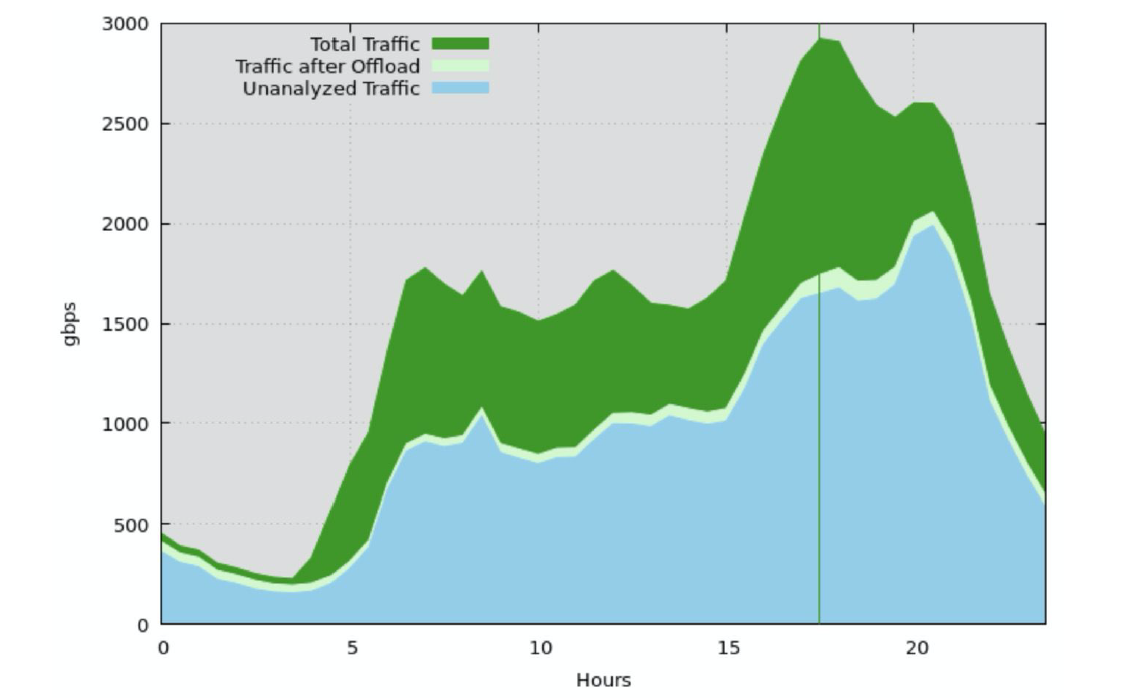
\includegraphics[width=15cm, height=7.2cm]{img/01_introduccio/trafic_peak.png}
        \caption[Trafic d'Internet]{\footnotesize{Volum de tràfic en un dia amb la sortida d'un nou videojoc. En blau el tràfic no analitzat,
        en ver fort el tràfic normal, en verd fluix el tràfic si la descarrega es fes amb multicast. Imatge d'Akamai.}}
    \end{figure}

    L'any 2015, el tràfic de serveis de vídeo en temps real, com Netflix, YouTube o Twitch, va representar pràcticament el 70\% del tràfic. Normalment,
    aquest tipus de tràfic va per pics, ja que quan una nova temporada d'una sèrie famosa, quan un youtuber important puja un nou vídeo o s'està
    fent un esdeveniment en directe la quantitat de gent veient el contingut sol augmentar de manera sobtada sobretot als primers moments. Això sol implicar
    en general problemes per donar accés a tothom al servei depenent de quanta gent sigui, mentre que al mateix temps altres serveis també es vegin
    afectats (les \ac{CDN} solen tenir molts serveis simultàniament distribuïts en microserveis).
    
    Per ficar dades i posar-nos en context del volum de tràfic, el màxim que s'ha arribat a donar simultàniament per part de la \ac{CDN} Akamai
    ha estat un pico de 167 Tbps en abril de 2020. Suposant un tràfic lineal, per simplificar, ja que normalment s'utilitzen codificacions \ac{CBR}
    en directe en temps real, amb una resolució de 1080p el tràfic és de 5 Mbps/connexió i fins a 20 Mbps/connexió en cas de 4k. Llavors, en 1080p
    suposant aquell tràfic màxim suportat llavors es podrien arribar fins a 33.4 milions de clients en 1080p i fins a 8.35 milions en 4k. Si tota
    Espanya volgués mirar un contingut en directe, seria impossible donar el servei.
    
    Aquests problemes de subministrament solen ser a causa que les connexions que es fan són punt a punt; dit d'una altra manera,
    són unicast. Això implica que el servei que pots donar en gran part està limitat al nombre de connexions simultànies que es pot donar. Malgrat que
    l'ús d'unicast té grans avantatges com la facilitat en la seguretat, la simplificació en l'arquitectura del programa o que pràcticament tots els
    dispositius del món suporten, també comporta un gran inconvenient.
    
    Si el contingut que has de distribuir als clients és exactament el mateix com en el cas de la televisió o la ràdio, unicast pot arribar a saturar
    un servei si el volum d'usuaris és molt alt. Arran d'aquesta qüestió de distribuir el mateix contingut a tothom que sol·licitàs, ja en
    els anys 80 amb la creació d'\ac{IP}, es va pensar en una tecnologia que soluciona aquests casos: \textbf{IP Multicast}. Malgrat no estar tan
    establerta com IP unicast, sí que la gran majoria de dispositius l'accepten.
    
    Per altra banda, al llarg dels anys, a les connexions unicast normalment han fet ús d'un protocol anomenat \ac{TCP}. Aquest protocol va ser especialment
    important en els anys 90 i a principis dels 2000 perquè Internet pogués funcionar i popularitzar-se, ja que les connexions eren lentes i poc fiables.
    Aquest protocol incorpora una sèrie de mecanismes per intentar pal·liar aquesta qüestió. No obstant això, amb la millora de les connexions i la seva fiabilitat
    hi ha altres protocols que poden ser més útils i millors en l'Internet que tenim actualment, incorporant funcionalitats que antigament no s'havien plantejat
    o que no semblaven rellevants. Un protocol que pareix que substituirà \ac{TCP} és QUIC, ja que millora bastant certs aspectes de TCP com l'establiment
    de la connexió molt més ràpidament (menys RTTs) o el fet de poder restablir la sessió amb el servidor en canviar de xarxa.
    
}

\subsection{Transfons del project}
{
    Aquest projecte es fa des de cero, encara agafa principalment dos projectes de codi lliure d'Internet i un borrador del \ac{IETF}:

    \begin{enumerate}
        \item{\textbf{\textit{Hypertext Transfer Protocol (\ac{HTTP}) over multicast QUIC}}, de Lucas Pardue, Richard Bradbury i Sam Hurst.}
        \item{\textbf{\textit{NGHQ}}: Llibrería escrita en C que implementa part de l'esborrany de \textit{\ac{HTTP} sobre multicast QUIC} fins la versió 7.}
        \item{\textbf{\textit{NGTCP2}}: Llibrería escrita en C que implementa el protocol QUIC segons l'estàndard escrit en el \ac{RFC} 9000.}
    \end{enumerate}

    La idea original ha estat de l'autor, encara que l'enfocament i la metodologia han estat proposades pel professor, Jorge Mata.

    Tot el codi utilitzat és de codi lliure desenvolupat per enginyers i que està pràcticament tot allotjat en plataformes
    online com Github. Tot el codi desenvolupat en aquest projecte està allotjat també al Github i també és de codi lliure.
}

\subsection{Objectius}
{
    El principal objectiu d'aquest projecte és desenvolupar un servidor de contingut en temps real que faci ús de la tecnologia
    QUIC sobre \ac{IP} multicast utilitzant la llibreria de software lliure. Al mateix temps, es pretén fer una comparativa de l'avantatge i inconvenients enfront del desenvolupament d'un servidor similar fent servir QUIC sobre IP unicast; és a dir, el perfil
    de QUIC genèric que proposa el \ac{RFC} 9000.

    El sistema estarà conformat per un servidor que rebrà peticions dels clients que demanaran el contingut de ràdio en directe a
    través d'\ac{IP}. Aquest servidor reencaminarà en el cas de multicast al flux multicast o enviarà directament la informació en
    cas d'unicast.

    \textbf{[ESBORRANY - FALTA L'IMATGE FINAL]}
    \begin{figure}[H]
        \label{fig:esborrany_configuracio}
        \centering
        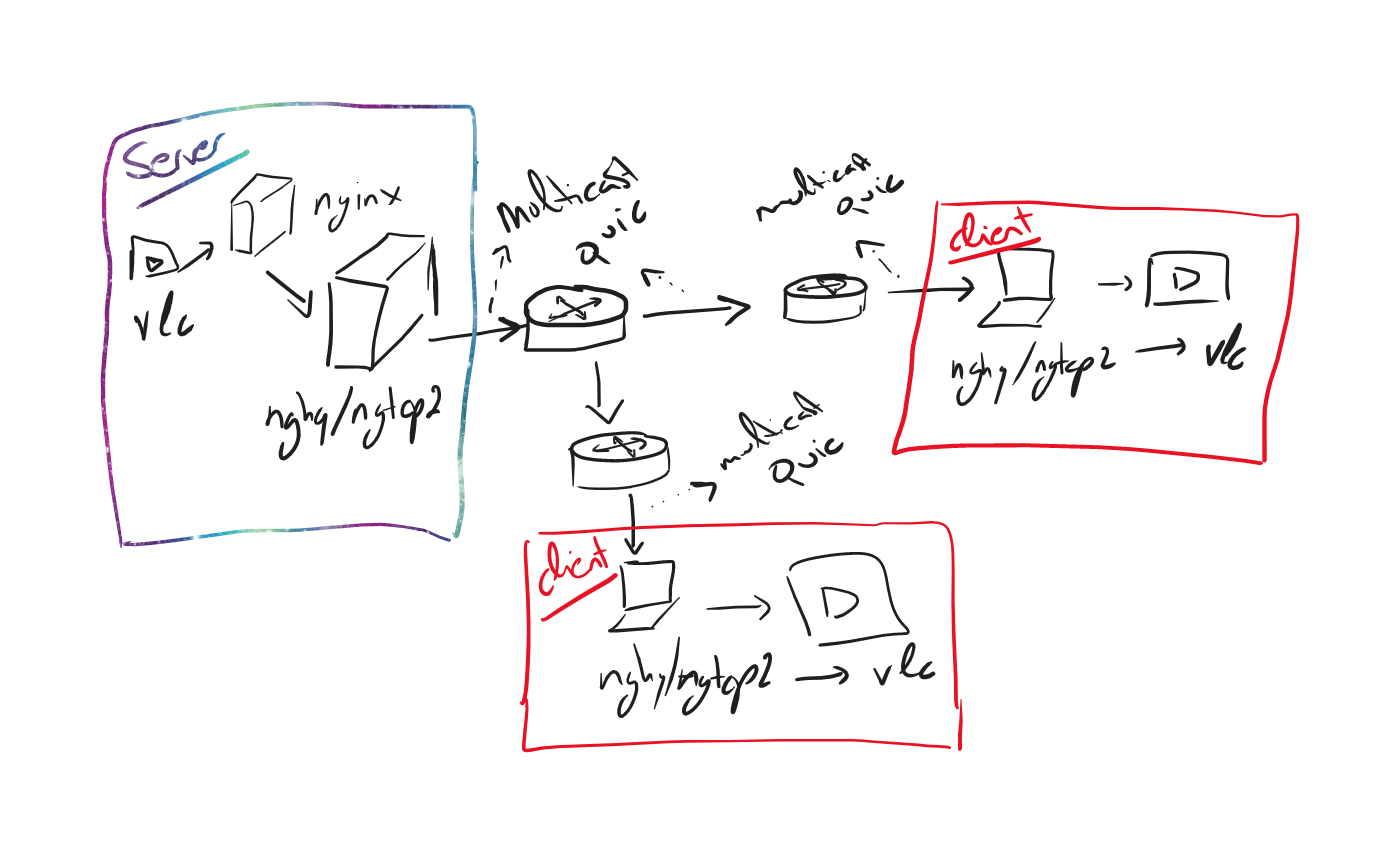
\includegraphics[width=15cm, height=7.2cm]{img/01_introduccio/topologia_conf.png}
        \caption[Trafic d'Internet]{\footnotesize{Topologia de la configuració plantejada.}}
    \end{figure}

    L'arquitectura del sistema està basada en el següent escenari: s'utilitzarà un reproductor d'àudio en directe, aquest serà captat
    per un servidor intermedi i li passarà el contingut al servidor que hem desenvolupat perquè el transmeti a través de la xarxa fins als
    clients perquè ho reprodueixin.
    
    El que es pretén demostrar és que hi ha un límit d'usuaris en el cas d'unicast i, en canvi, no hi ha un límit en el cas d'usuaris multicast.
    Donat que la majoria de la gent accedeix a través d'HTTP als serveis d'aquest tipus de contingut es farà ús de QUIC, un protocol desplegat
    pensat en HTTP. Cal indicar que QUIC permet l'ús de fils simultanis que es faran servir per enviar tràfic també a través de multicast. El perfil
    de QUIC en el cas de multicast difereix en alguns paràmetres i configuracions d'un perfil de QUIC normal.
}

\subsection{Requeriments i especificacions}
{
    \textbf{Requeriments del projecte}:
    \begin{itemize}
        \item Proveir un sistema integrat de transmissió de contingut en directe tant per la part del client
        com la part del servidor que permiti la transmissió via unicast i/o multicast.
        \item Donar una guia als usuaris finals per fer la instal·lació tan simple com sigui possible (annexe?)
        \item Tot el software extern o implementat ha de ser gratuït i de codi lliure.
        \item Evaluar la solució final emulant-la en diferents escenaris i proveir uns resultats consistents.
        \item La transferència del contingut ha de ser en el màxim possible fluid i continua.
        \item El software desenvolupat ha de ser el més flexible possible per poder utilitzar-lo en futures
        implementacions d'altres softwares si es volgués.
        \item S'ha de poder avaluar el tràfic de manera quantitativa i qualitativa.
    \end{itemize}
    
    \textbf{Especificacions del projecte}:
    \begin{itemize}
        \item Hi ha d'haver com a mínim dos clients reben el contingut, ja que si no multicast deixa de tenir sentit encara
        que és viable fer-ho per un.
        \item El mostreig de la ràdio ha de poder variar durant la transmissió.
        \item Per avaluar el sistema en un entorn controlat, el servidor i els clients seran màquines virtual Linux que corren
        damunt el mateix sistema operatiu; Linux també.
        \item S'avaluarà el tràfic amb eines d'ús extensiu, proveint els filtres necessaris per descodificar els missatges transmesos.
    \end{itemize}
}

\subsection{Pla de feina}
{
    En aquesta secció de document es descriu en detall tots els blocs de treball en el qual s'ha dividit la feina i els temps (Diagrama de Gantt)
    en els que s'ha fet la tasca corresponent.
    
    Al llarg del projecte, hi ha hagut diversos canvis en respecte al pla original. Els principals canvis han estat els següents:
    \begin{itemize}
        \item \textbf{Lectura de \ac{RFC}s}. Donat la complexitat del projecte i la profunditat d'aquest s'ha vist que la quantitat de documentació
        al respecte que s'ha hagut de llegir ha estat molt major de la qual s'esperava, en gran part, ja que el nombre de tecnologies
        necessaries per poder entendre i desenvolupar una plataforma com la que es demana és molt major del qual es podria esperar a priori.
        També, a causa que s'utilitzen tecnologies noves com QUIC, hi ha hagut \ac{RFC}s que han aparegut durant el transcurs com el 9221.
        \item \textbf{Certs programes no existien o no compilaven}. Per fer l'escenari de proves s'ha volgut fer servir un software nou per virtualitzar
        la xarxa intentant imitar la de la pràctica \ac{IP} multicast de l'assignatura \ac{TCGI} del grau d'Enginyeria de serveis i sistemes
        de telecomunicaciones del \ac{ETSETB}. Es va trobar que les màquines virtuals i el software utilitzat en aquelles màquines és antic i qualcun
        ja no està disponible. S'ha buscat alternatives al respecte.
        
        El que més ha dificultat i endarrerit el desenvolupament ha estat la lectura de la documentació, ja que era molt més extensa del que s'esperava a priori
        a més que també entrava en molts detalls que semblaven contradictoris amb la idea, encara que sembla que no. S'ha de pensar que la proposta és una
        tecnologia que encara no s'ha desenvolupat del tot i encara està en procés, llavors això és més una prova del concepte que una demostració per ficar-ho
        a producció. Encara s'està lluny d'aquest punt com es veurà al llarg del treball.
    \end{itemize}
}
\subsubsection{Estructura de la feina}
{
    \textbf{[ESBORRANY - FALTA L'IMATGE FINAL]}
    \begin{figure}[H]
        \label{fig:estructura}
        \centering
        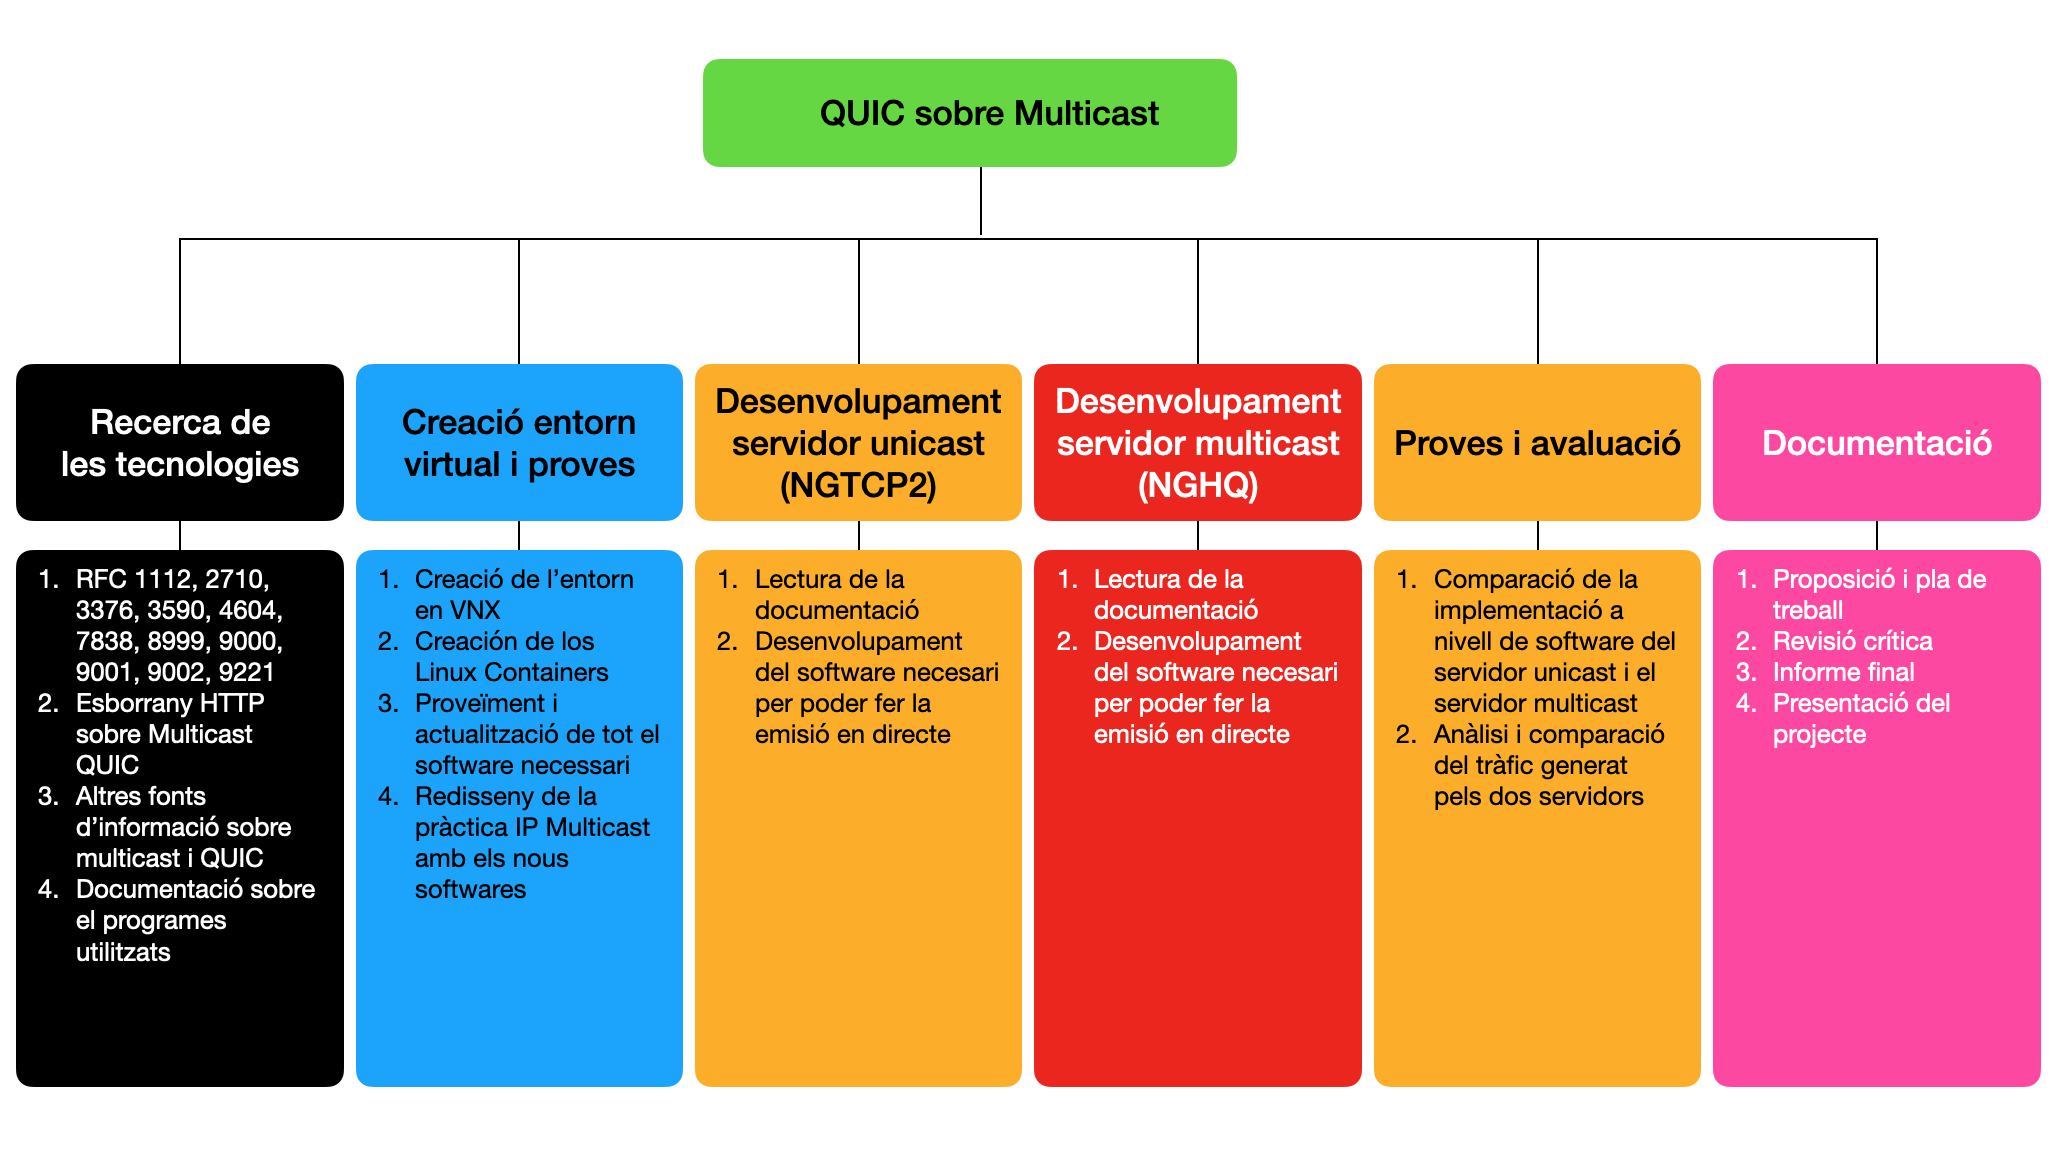
\includegraphics[width=15cm]{img/01_introduccio/estructura_treball.png}
    \end{figure}
}
\subsubsection{Paquets de feina, tasques i fites}
{
    \begin{center}
        
\begin{table}[H]
    \begin{tabular}{|l|ll|l}
    \cline{1-3}
    Projecte: \textbf{Recerca de les tecnologies}                                                                                                                                                                                                                                          & \multicolumn{2}{l|}{WP ref: \textbf{WP1}}                                                                                                                                               &  \\ \cline{1-3}
    Element principal: Lectura de la documentació                                                                                                                                                                                                                                                      & \multicolumn{2}{l|}{Pàg. 1 de 6}                                                                                                                                               &  \\ \cline{1-3}
    \multirow{2}{*}{\begin{tabular}[c]{@{}l@{}}Breu descripció: \\ Lectura del RFCs necessaris per tal d'entendre i proposar\\ solucions adequades per crear un perfil de QUIC sobre\\ multicast.\\ \\ Lectura de la documentació necesaria\end{tabular}}                                            & \multicolumn{2}{l|}{\begin{tabular}[c]{@{}l@{}}Data d'inici estimada:\\              01-10-2021 \\ Data de finalització estimada: \\                01-11-2021\end{tabular}} &  \\ \cline{2-3}
                                                                                                                                                                                                                                                                                                       & \multicolumn{2}{l|}{\begin{tabular}[c]{@{}l@{}}Data d'inici real:\\                14-09-2021 \\ Data de finalització real:\\           30-04-2022\end{tabular}}        &  \\ \cline{1-3}
    \begin{tabular}[c]{@{}l@{}}Tasques internes:\\ \\ T1. RFC 1112, 2710, 3376, 3590, 4604, 7838, 8999,\\        9000, 9001, 9002, 9221\\ T2. Esborrany HTTP sobre Multicast QUIC\\ T3. Altres fonts d'informació sobre multicast i QUIC\\ T4. Documentació sobre el programes utilitzats\end{tabular} & \multicolumn{1}{l|}{\begin{tabular}[c]{@{}l@{}}Entregables:\\ Tasca 1 i 2\end{tabular}}    & \begin{tabular}[c]{@{}l@{}}Dates:\\ incluides\\ en el\\ document\end{tabular}    &  \\ \cline{1-3}
    \end{tabular}
    \end{table}
        \begin{table}[H]
    \begin{tabular}{|l|ll|l}
    \cline{1-3}
    Projecte: \textbf{Creació entorn virtual i proves}                                                                                                                                                                                                                                          & \multicolumn{2}{l|}{WP ref: \textbf{WP2}}                                                                                                                                                                   &  \\ \cline{1-3}
    Element principal: Entorn virtual                                                                                                                                                                                                                                              & \multicolumn{2}{l|}{Pàg. 2 de 6}                                                                                                                                                                   &  \\ \cline{1-3}
    \multirow{2}{*}{\begin{tabular}[c]{@{}l@{}}Breu descripció: \\ Creació de l'entorn virtual amb VNX, proveïment \\ de les màquines virtuals amb el software necesari i\\ fer la pràctica d'IP multicast de TCGI per testejar\\ que l'entorn funciona correctament\end{tabular}}   & \multicolumn{2}{l|}{\begin{tabular}[c]{@{}l@{}}Data d'inici estimada:\\               16-09-2021\\  Data de finalització estimada:\\                10-10-2021\end{tabular}}                     &  \\ \cline{2-3}
                                                                                                                                                                                                                                                                                       & \multicolumn{2}{l|}{\begin{tabular}[c]{@{}l@{}}Data d'inici real:\\                16-09-2021\\ Data de finalització real:\\                30-12-2022\end{tabular}}                            &  \\ \cline{1-3}
    \begin{tabular}[c]{@{}l@{}}Tasques internes:\\ \\ T1. Creació de l'entorn en VNX\\ T2. Creació dels Linux Containers\\ T3. Proveïment i actualització de tot el software\\       necessari\\ T4. Rediseny de la pràctica IP Multicast amb \\       els nous softwares\end{tabular} & \multicolumn{1}{l|}{\begin{tabular}[c]{@{}l@{}}Entregables:\\ Presentació al\\ professor de \\ l'escenari\\ montat\end{tabular}} & \begin{tabular}[c]{@{}l@{}}Dates:\\ 14-01-2022\\ \end{tabular} &  \\ \cline{1-3}
    \end{tabular}
    \end{table}
        \begin{table}[H]
    \begin{tabular}{|l|ll|l}
    \cline{1-3}
    \begin{tabular}[c]{@{}l@{}}Projecte: \textbf{Desenvolupament servidor} \\                \textbf{unicast (NGTCP2)}\end{tabular}                                                                                                                                  & \multicolumn{2}{l|}{WP ref: \textbf{WP3}}                                                                                                                                            &  \\ \cline{1-3}
    Element principal: Desenvolupament de software                                                                                                                                                                                                 & \multicolumn{2}{l|}{Pàg. 3 de 6}                                                                                                                                            &  \\ \cline{1-3}
    \multirow{2}{*}{\begin{tabular}[c]{@{}l@{}}Breu descripció:\\ \\ Creació d'un servidor unicast que utilitzi el protocol\\ QUIC per poder utilitzar-lo per comparar amb un\\ que utilitzi multicast. També s'ha de fer el client.\end{tabular}} & \multicolumn{2}{l|}{\begin{tabular}[c]{@{}l@{}}Data d'inici estimada:\\               01-11-2021\\ Data de finalització estimada:\\                01-12-2021\end{tabular}} &  \\ \cline{2-3}
                                                                                                                                                                                                                                                   & \multicolumn{2}{l|}{\begin{tabular}[c]{@{}l@{}}Data d'inici real:\\                15-02-2022\\ Data de finalització real:\\                05-05-2022\end{tabular}}        &  \\ \cline{1-3}
    \begin{tabular}[c]{@{}l@{}}Tasques internes:\\ \\ T1. Lectura de la documentació\\ T2. Desenvolupament del software necesari per poder\\        per poder fer la emisió en directe.\end{tabular}                                               & \multicolumn{1}{l|}{\begin{tabular}[c]{@{}l@{}}Entregables:\\ Tasca 1\\ Tasca 2\\ Tasca 3\end{tabular}}   & \begin{tabular}[c]{@{}l@{}}Dates:\\ 15-05-2022\end{tabular}   &  \\ \cline{1-3}
    \end{tabular}
    \end{table}
        \begin{table}[H]
    \begin{tabular}{|l|ll|l}
    \cline{1-3}
    \begin{tabular}[c]{@{}l@{}}Projecte: \textbf{Desenvolupament servidor} \\                \textbf{multicast (NGHQ)}\end{tabular}                                                                                                                                  & \multicolumn{2}{l|}{WP ref: \textbf{WP4}}                                                                                                                                            &  \\ \cline{1-3}
    Element principal: Desenvolupament de software                                                                                                                                                                                                 & \multicolumn{2}{l|}{Pàg. 4 de 6}                                                                                                                                            &  \\ \cline{1-3}
    \multirow{2}{*}{\begin{tabular}[c]{@{}l@{}}Breu descripció:\\ \\ Creació d'un servidor multicast que utilitzi el protocol\\ QUIC per poder utilitzar-lo per comparar amb un\\ que utilitzi unicast. També s'ha de fer el client.\end{tabular}} & \multicolumn{2}{l|}{\begin{tabular}[c]{@{}l@{}}Data d'inici estimada:\\               01-11-2021\\ Data de finalització estimada:\\                01-12-2021\end{tabular}} &  \\ \cline{2-3}
                                                                                                                                                                                                                                                   & \multicolumn{2}{l|}{\begin{tabular}[c]{@{}l@{}}Data d'inici real:\\                15-02-2022\\ Data de finalització real:\\                05-05-2022\end{tabular}}        &  \\ \cline{1-3}
    \begin{tabular}[c]{@{}l@{}}Tasques internes:\\ \\ T1. Lectura de la documentació\\ T2. Desenvolupament del software necesari per poder\\        per poder fer la emisió en directe.\end{tabular}                                               & \multicolumn{1}{l|}{\begin{tabular}[c]{@{}l@{}}Entregables:\\ Tasca 1\\ Tasca 2\\ Tasca 3\end{tabular}}   & \begin{tabular}[c]{@{}l@{}}Dates:\\ 15-05-2022\end{tabular}   &  \\ \cline{1-3}
    \end{tabular}
    \end{table}
        % Please add the following required packages to your document preamble:
% \usepackage{multirow}
\begin{table}[H]
    \begin{tabular}{|l|ll|l}
    \cline{1-3}
    Projecte: \textbf{Proves i avaluació}                                                                                                                                                                                                              & \multicolumn{2}{l|}{WP ref: \textbf{WP5}}                                                                                                                                            &  \\ \cline{1-3}
    Element principal: Simulació i proves de qualitat                                                                                                                                                                                         & \multicolumn{2}{l|}{Pàg. 5 de 6}                                                                                                                                            &  \\ \cline{1-3}
    \multirow{2}{*}{\begin{tabular}[c]{@{}l@{}}Breu descripció:\\ \\ Totes les simulacions i  avaluacions necessaries\\ per aconseguir proves concloents de en quin cas\\ és millor utilitzar unicast i quin multicast.\end{tabular}}         & \multicolumn{2}{l|}{\begin{tabular}[c]{@{}l@{}}Data d'inici estimada:\\               01-11-2021\\ Data de finalització estimada:\\                15-12-2021\end{tabular}} &  \\ \cline{2-3}
                                                                                                                                                                                                                                              & \multicolumn{2}{l|}{\begin{tabular}[c]{@{}l@{}}Data d'inici real:\\                15-02-2022\\ Data de finalització real:\\                05-05-2022\end{tabular}}        &  \\ \cline{1-3}
    \begin{tabular}[c]{@{}l@{}}Tasques internes:\\ \\ T1. Comparació de l'implementació a nivell de\\ software del servidor unicast i el servidor\\ multicast\\ T2. Anàlisi i comparació del tràfic generat pels\\ dos servidors\end{tabular} & \multicolumn{1}{l|}{\begin{tabular}[c]{@{}l@{}}Entregables:\\ Tasca 1\\ Tasca 2\\ Tasca 3\end{tabular}}   & \begin{tabular}[c]{@{}l@{}}Dates:\\ 15-05-2022\end{tabular}   &  \\ \cline{1-3}
    \end{tabular}
    \end{table}
        % Please add the following required packages to your document preamble:
% \usepackage{multirow}
\begin{table}[H]
    \begin{tabular}{|l|ll|l}
    \cline{1-3}
    Projecte: \textbf{Documentació}                                                                                                                                                                                          & \multicolumn{2}{l|}{WP ref: \textbf{WP6}}                                                                                                                                                                     &  \\ \cline{1-3}
    Element principal: Documentació                                                                                                                                                                                 & \multicolumn{2}{l|}{Pàg. 6 de 6}                                                                                                                                                                     &  \\ \cline{1-3}
    \multirow{2}{*}{\begin{tabular}[c]{@{}l@{}}Breu descripció:\\ \\ Documentació que s'ha d'entregar. Un manual\\ d'usuari per poder configurar ambdos servidors\\ serà inclós en el document final.\end{tabular}} & \multicolumn{2}{l|}{\begin{tabular}[c]{@{}l@{}}Data d'inici estimada:\\               15-09-2021\\ Data de finalització estimada:\\                15-01-2022\end{tabular}}                          &  \\ \cline{2-3}
                                                                                                                                                                                                                    & \multicolumn{2}{l|}{\begin{tabular}[c]{@{}l@{}}Data d'inici real:\\                20-01-2022\\ Data de finalització real:\\                15-05-2022\end{tabular}}                                 &  \\ \cline{1-3}
    \begin{tabular}[c]{@{}l@{}}Tasques internes:\\ \\ T1. Proposició i pla de treball\\ T2. Revisió crítica\\ T3. Informe final\\ T4. Presentació del projecte\end{tabular}                                         & \multicolumn{1}{l|}{\begin{tabular}[c]{@{}l@{}}Entregables:\\ Tasca 1\\ Tasca 2\\ Tasca 3\end{tabular}} & \begin{tabular}[c]{@{}l@{}}Dates:\\ 08-10-21\\ 30-11-21\\ 15-05-22\\ 28-05-22\end{tabular} &  \\ \cline{1-3}
    \end{tabular}
    \end{table}
    \end{center}
    \newpage
    \textbf{Objectius}
    \begin{table}[H]
    \begin{tabular}{|l|l|l|l|l|}
    \hline
    \textbf{WP\#} & \textbf{Tasca\#} & \textbf{Títol curt}                                                                                                                               & \textbf{Objectius/Entregables}                                                                                                                       & \textbf{Data (setmana)}                                         \\ \hline
    WP1           & T1               & \begin{tabular}[c]{@{}l@{}}RFC 1112, 2710, 3376,\\ 4604, 7838, 8999,\\ 9001, 9002, 9221\end{tabular}                                              & Estat de l'art                                                                                                                                       & \begin{tabular}[c]{@{}l@{}}Inclós en el\\ document\end{tabular} \\ \hline
    WP1           & T1               & \begin{tabular}[c]{@{}l@{}}Esborrany HTTP sobre\\ Multicast QUIC\end{tabular}                                                                     & Estat de l'art                                                                                                                                       & \begin{tabular}[c]{@{}l@{}}Inclós en el\\ document\end{tabular} \\ \hline
    WP1           & T1               & \begin{tabular}[c]{@{}l@{}}Altres fonts\\ d'informació sobre\\ multicast i QUIC\end{tabular}                                                      & Estat de l'art                                                                                                                                       & \begin{tabular}[c]{@{}l@{}}Inclós en el\\ document\end{tabular} \\ \hline
    WP1           & T2               & \begin{tabular}[c]{@{}l@{}}Documentació sobre\\ el programes utilitzats\end{tabular}                                                              & Guies                                                                                                                                                & \begin{tabular}[c]{@{}l@{}}Inclós en el\\ document\end{tabular} \\ \hline
    WP2           & T2               & \begin{tabular}[c]{@{}l@{}}Creació de l'entorn\\ en VNX\end{tabular}                                                                              & Entorn virtual montat                                                                                                                                & \begin{tabular}[c]{@{}l@{}}Setmanes \\ 37 a 52\end{tabular}     \\ \hline
    WP2           & T2               & \begin{tabular}[c]{@{}l@{}}Creació de los Linux\\ Containers\end{tabular}                                                                         & \begin{tabular}[c]{@{}l@{}}Màquines disponibles\\ per l'entorn virtual\end{tabular}                                                                  & \begin{tabular}[c]{@{}l@{}}Setmanes\\ 37 a 52\end{tabular}      \\ \hline
    WP2           & T2               & \begin{tabular}[c]{@{}l@{}}Proveïment i\\ actualització de tot el\\ software necessari\end{tabular}                                               & \begin{tabular}[c]{@{}l@{}}Màquines provistes\\ del software requerit\end{tabular}                                                                   & \begin{tabular}[c]{@{}l@{}}Setmanes\\ 37 a 52\end{tabular}      \\ \hline
    WP2           & T2               & \begin{tabular}[c]{@{}l@{}}Redisseny de la\\ pràctica IP Multicast\\ amb els nous softwares\end{tabular}                                          & \begin{tabular}[c]{@{}l@{}}Comentaris per actualitzar\\ la pràctica d'IP Multicast\\ amb software actual\\ (annexe)\end{tabular}                     & \begin{tabular}[c]{@{}l@{}}Setmanes\\ 37 a 52\end{tabular}      \\ \hline
    WP3           & T1               & \begin{tabular}[c]{@{}l@{}}Lectura de la\\ documentació\\ (NGTCP2)\end{tabular}                                                                   & \begin{tabular}[c]{@{}l@{}}Explicació del software\\ a estat de l'art\end{tabular}                                                                   & \begin{tabular}[c]{@{}l@{}}Setmanes\\ 7 a 19\end{tabular}       \\ \hline
    WP3           & T3               & \begin{tabular}[c]{@{}l@{}}Desenvolupament del\\ software necesari\\ per poder fer la emisió\\ en directe\end{tabular}                            & \begin{tabular}[c]{@{}l@{}}Creació del servidor per\\ enviar la radio IP via\\ unicast\end{tabular}                                                  & \begin{tabular}[c]{@{}l@{}}Setmanes\\ 7 a 19\end{tabular}       \\ \hline
    WP4           & T1               & \begin{tabular}[c]{@{}l@{}}Lectura de la\\ documentació\end{tabular}                                                                              & \begin{tabular}[c]{@{}l@{}}Explicació del software\\ a l'estat de l'art\end{tabular}                                                                 & \begin{tabular}[c]{@{}l@{}}Setmanes\\ 7 a 19\end{tabular}       \\ \hline
    WP4           & T3               & \begin{tabular}[c]{@{}l@{}}Desenvolupament del\\ software necesari\\ per poder fer la emisió \\ en directe\end{tabular}                           & \begin{tabular}[c]{@{}l@{}}Creació del servidor per \\ enviar la radio IP via\\ multicast\end{tabular}                                               & \begin{tabular}[c]{@{}l@{}}Setmanes\\ 7 a 19\end{tabular}       \\ \hline
    \end{tabular}
\end{table}
    \begin{table}[H]
    \begin{tabular}{|l|l|l|l|l|}
    \hline
    \textbf{WP\#} & \textbf{Tasca\#} & \textbf{Títol curt}                                                                                                                               & \textbf{Objectius/Entregables}                                                                                                                       & \textbf{Data (setmana)}                                         \\ \hline 
    WP5           & T4               & \begin{tabular}[c]{@{}l@{}}Comparació de la\\ implementació a \\ nivell de software\\ del servidor unicast i\\ el servidor multicast\end{tabular} & \begin{tabular}[c]{@{}l@{}}Explicació de les\\ avantages i incovenients\\ del desenvolupament a\\ l'apartat de resultats del\\ document\end{tabular} & \begin{tabular}[c]{@{}l@{}}Setmanes\\ 7 a 19\end{tabular}       \\ \hline
    WP5           & T4               & \begin{tabular}[c]{@{}l@{}}Anàlisi i comparació\\ del tràfic generat pels\\ dos servidors\end{tabular}                                            & \begin{tabular}[c]{@{}l@{}}Gràfica comparativa de\\ la quantitat de tràfic\\ generat per les dues\\ implementacions\end{tabular}                     & \begin{tabular}[c]{@{}l@{}}Setmanes\\ 7 a 19\end{tabular}       \\ \hline   
    WP6           & T1               & \begin{tabular}[c]{@{}l@{}}Proposició i pla de\\ treball\end{tabular}                                                                             & Proposió i pla de treball                                                                                                                            & Setmana 37                                                      \\ \hline
    WP6           & T2               & Revisió Crítica                                                                                                                                   & Revisió Crítica                                                                                                                                      & Setmana 48                                                      \\ \hline
    WP6           & T3               & Informe final                                                                                                                                     & Informe final                                                                                                                                        & Setmana 19                                                      \\ \hline
    WP6           & T4               & \begin{tabular}[c]{@{}l@{}}Presentació del\\ projecte\end{tabular}                                                                                & Presentació del projecte                                                                                                                             & Setmana 20                                                      \\ \hline
    \end{tabular}
\end{table}
}
\subsection{Diagrama temporal (Diagrama de Gantt)}
{
    \label{ssec:gantt}
    \begin{figure}[H]
        \centering
        %\includegraphics[width=13cm]{img/diagram_gantt.png}
        \begin{adjustbox}{max totalsize={\textwidth}{.8\textheight},center}
    \begin{ganttchart}[
        hgrid,
        vgrid={*{6}{draw=none},{dotted}},
        vrule/.style={very thick, red},
        x unit=0.125cm,
        time slot format=isodate,
        time slot unit=day,
        calendar week text = {W\currentweek{}},
        bar height = 0.6, %necessary to make it fit the height
        bar top shift = 0.2, %to move it inside the grid space ;)
        bar label node/.append style={align=left,text width={width("Desenvolupament ")}},
        bar incomplete/.append style={fill=cyan},
        progress label text = \relax
        ]{2021-09-13}{2022-06-05}
        \gantttitlecalendar{year, month=name, week} \\
        \ganttbar[bar/.append style={fill=cyan}]{RFCs}{2021-09-15}{2022-05-01}\\
        \ganttbar[bar/.append style={fill=blue}]{Draft}{2021-09-15}{2021-10-01}\\
        \ganttbar[bar/.append style={fill=cyan}]{multicast \& \\ QUIC}{2021-09-15}{2022-05-01}\\
        \ganttbar[bar/.append style={fill=blue}]{Documentació \\ programes}{2021-09-15}{2021-12-31}\\
        \ganttbar[bar/.append style={fill=cyan}]{Entorn VNX}{2021-09-15}{2021-12-31}\\
        \ganttbar[bar/.append style={fill=blue}]{LXCs}{2021-10-15}{2021-12-31}\\
        \ganttbar[bar/.append style={fill=cyan}]{Provisionament}{2021-10-15}{2021-12-31}\\
        \ganttbar[bar/.append style={fill=blue}]{Pràctica}{2021-10-15}{2021-12-31}\\
        \ganttbar[bar/.append style={fill=cyan}]{Documentació \\ NGTCP2}{2022-02-15}{2022-05-15}\\
        \ganttbar[bar/.append style={fill=blue}]{Desenvolupament \\ NGTCP2}{2022-02-15}{2022-05-15}\\
        \ganttbar[bar/.append style={fill=cyan}]{Documentació \\ NGHQ}{2022-02-15}{2022-05-15}\\
        \ganttbar[bar/.append style={fill=blue}]{Desenvolupament \\ NGHQ}{2022-02-15}{2022-05-15}\\
        \ganttbar[bar/.append style={fill=cyan}]{Comparativa \\ desenvolupament}{2022-02-15}{2022-05-15}\\
        \ganttbar[bar/.append style={fill=blue}]{Comparativa \\ tràfic}{2022-04-10}{2022-04-20}\\
        \ganttbar[bar/.append style={fill=cyan}]{Proposició}{2021-09-15}{2021-09-20}\\
        \ganttbar[bar/.append style={fill=blue}]{Revisió}{2021-11-10}{2021-11-15}\\
        \ganttbar[bar/.append style={fill=cyan}]{Informe}{2022-04-05}{2022-05-15}\\
        \ganttbar[bar/.append style={fill=blue}]{Presentació}{2022-05-10}{2022-05-30}\\
        %\ganttvrule{2022-05-15}{2022-05-15}
    \end{ganttchart}
\end{adjustbox}
        \caption[Diagrama de Gantt del projecte]{\footnotesize{Diagrama de Gantt del projecte}}
        \label{fig:gantt}
    \end{figure}
}


\clearpage

%%% StateOfTheArt %%%
\section{Live-streaming state of art }

{
    Live-streaming content is in its dawn. Although it is possible and it is being done nowadays, real-time content in Internet is still primitive
    in the way we are delivering it. We are using brute-force to deliver huge amounts of real-time content. It is a matter of fact that 
    the demand for this type of content is growing far faster than the CDN \footnote{CDN: Content Delivery Network} (from now on called servers)
    are able to supply to the spectactors (from now on called clients).
    
    Even though someone might say it is almost every content via internet, there are still a lot of events that can not transmitted using internet 
    because it cannot be supported\footnote{https://github.com/GrumpyOldTroll/wicg-multicast-receiver-api/blob/master/explainer.md} due to the heavy load
    of users that need to managed. As Jake Holland from Akamai wrote on Github: "The capacity of CDNs and others to deliver popular content at scale is 
    not keeping up with demand."

    In april of 2020, Akamai achieved the new world record of peak traffic delivery which was 176 tbps. It seems a lot, however it is not. Making some linear
    and quick easy maths it is easy to see that it is not. Keeping in mind that usually for real-time video we use CBR\footnote{Constant Bit-Rate} encoder in
    order to squeeze the internet resources, for a 1080p video we need a bit-rate of 5 mbps, and for a 4k video, 20 mbps. This means that with the current
    world-record we can arrive to 35.2 millions of simultaneous users for live-streaming content using a 1080p encoding and 8.8 millions users using 4k.
    Considering that the world population with internet access is 5200 million people we are really faraway from delivering TV or Radio via Internet using
    the current methods. What is more, the Fifa World Cup Finals 2018 were seen by 500 million people, 200 million to 300 million people were seeing in India the Cricket
    World Cup in 2015 (whenever India is playing) and a large etcetera with a lot of content can be done.  The brute force does not seem like a good stategy for scaling 
    anymore, maybe only for quick deployments.

    The solution that is being discussed in this Final Degree Project proposes to use multicast instead of unicast in order to avoid this scalability limitation, due to
    the fact that using this technology for distribute the same content to everyone is more efficient in terms of computation in the servers and of resources in general.
}

\subsection{Technologies used at the moment}
{
    TCP is at the moment the main protocol over Internet. Almost every service at the moment uses it and HTTP is not an exception. When doing a HTTP request or response (versions 1.0,
    1.1 and 2), TCP is being used. Even though, it is almost 50 years old and the internet has evolved and has grown significantly, it is still the main protocol. However, it is reaching
    its full capacity in two particular scenarios: websites with small pageload and real-time content such as TV and Radio. Although, the main goal of this project is to focus on the 
    real-time content delivery, the small pageload problem will also be explained briefly because is what QUIC tries to solve as originally planned.    
    
    Most of the is requested via a navigator like Firefox or Google Chrome, which use the HTTP protocol as the main communication protocol which the use of TCP. It is clear and obvious
    that for large content which is not in real-time that can be stored like films, TCP is not a big bottleneck. However, in the last several years, with the
    raising of important services (like e-commerce) and cyberattacks, specially spoofing, the use of TLS\footnote{TLS : Transport Security Layer} has also became a standard. Websites that
    deliver real-time video like Youtube or Twitch are not an exception either. This also adds some complexity and workload delivering the website to the client.

    When someone connects to a internet using a web-browser at least it need 3 packets for for stablishing the TCP connection, 3 for stablishing the TLS connection over 
    TCP and 2 HTTP packets (request and response).It is being received the first byte of content after the 7th packet! This handshake, although being the most being used,
    it is not optimal. When a really small website is being delivered (imagine an html "Hello World!"), a load of resources and packets are being used for a deliver a 
    small packet. More control stuff than content. It gets even worse, if it is the case that have already stablished a connection earlier and after a while there
    is a new request; all this handshake has to be done again because TCP and TLS are a connection oriented protocols, but HTTP is not. QUIC aims to solve this type of problems.
}
\subsection{The new standard: QUIC}
{
    The main goal of QUIC is not only to stablish the connection as fast as possible requiring the minimum packets until the first byte of content is sent but 
    also do all of this in a secure way. The initials draft were done by Google using the acronym QUIC for Quick UDP Internet Protocol, although nowadays is a RFC (RFC 9000) which
    has been done by the IETF\footnote{Internet Engineering Task Force} and it is not an acronym anymore.

    TCP has been so popular that has been implemented on most of the kernels and this is a problem. Nevertheless, there is another protocol that is really simple in terms of what
    it does because it passes almost all responsabilities to the upper layers: UDP\footnote{Unit Datagram Protocol}. It is not that extended in terms of use, but almost all kernels
    also implemented. In the past decades, many firewalls did not allow the pass of UDP packets because 




    It is clear and obvious that for large content that can be stored in a small buffer and does not need to be real-time we can use a really known 
    protocol that have been around for years which is TCP. It is the main protocol for most of the services in the internet and has been even implemented
    in the kernel of most of the devices. Many of the devices that rule internet like firewalls or load-balancers were designed bearing in mind that the
    protocol that had to be used was TCP. During many years it was not a priority to use other transport layer protocols except in rare case.

    Nowadays, might be surprising that we use that procotol that is end-to-end to deliver the same real-time content to a large amount of spectactors (for
    now on they will be called clients)\footnote{In the Annexe I there is a larger explanation and details on how to test this with famous websites at the
    moment}. It is easy to see that this approach although having many withdrawals it has some benefits.

    The solution that is being discussed in this Final Degree Project proposes to use multicast instead of unicast in order to avoid this scalability limitation, due to
    the fact that using this technology for distribute the same content to everyone is more efficient in terms of computation in the servers and of resources in general.
}

\subsection{Benefits of using TCP for live-streaming}
{
    The main benefit with this approach for real-time content is the easiness on the programming and mounting at first time. All devices (or almost all) can
    bypass internet elements when they talk TCP. 
 
    
    At the current moment, it is the standard which means less complexity, more tools and easier to implement. For
    young services that are not expected to growth a lot TCP is more than enought for most cases.

    At the same time, there 
}

\subsection{UDP}{
    
    Nevertheless, in the last decade it has been a growing interest in other procotols that are end-to-end and allow to expand functionalities in upper layers:
    UDP\footnote{UDP: User Datagram Protocol}. It is a really simple protocol with almost 0 functionalities aside from passing the content to the upper layer.
    It has been around since the creation of the internet. That means, like with TCP, is implemented in the kernel. Changing the kernel of all the devices in
    the internet it is imposible 
}

\subsection{Topic}

Here you have a couple of references about LaTeX ~\cite{latexcompanion} and electrodynamics \cite{einstein}.

\bigskip

\subsection{Topic}


\clearpage

%%% METHODOLOGY %%%
\section{Metodologia}
\subsection{Entorn de proves}
{
    L'entorn de proves s'ha creat amb el software VNX. L'escenari està basat en l'entorn de la pràctica d'IP Multicast
    de l'assignatura de TCGI, ja que és un entorn conegut, ademés de ser suficient per fer la demostració i ser
    lleuger a l'hora de fer modificacions i montar-ho l'ordinador base.

    Totes les màquines virtuals de l'entorn son una rèplica d'un LXC amb el sistema operatiu Ubuntu 18.04 LTS.
    Aquest està provisionat amb tot el software necessari tant pels routers com pels hosts. En el cas de precisar un
    software en desenvolupament, com pot ser els scripts per fer correr el servidor i els clients, llavors
    també es poden copiar al montar l'escenari (VNX permet copiar carpeta especifiques al terminal indicat).

    \begin{figure}[H]
        \label{fig:network}
        \centering
        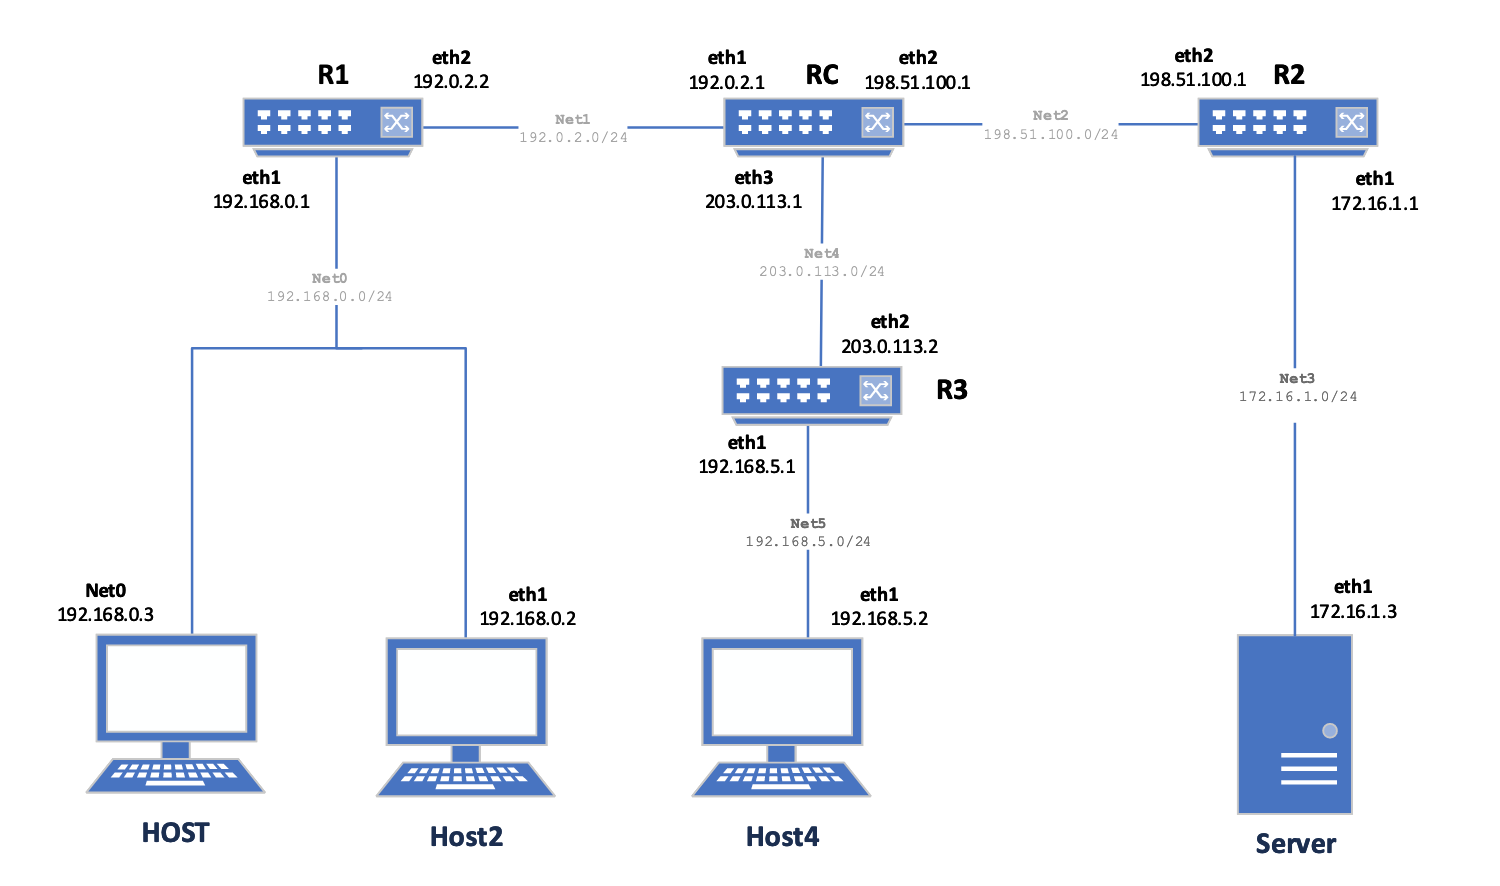
\includegraphics[width=15cm]{img/03_metodologia/network_topology.png}
    \end{figure}

    La topologia de xarxa consisteix en 3 hosts, 2 virtuals i un real (HOST), que rebran la retransmissió;
    4 routers que s'encarreguen de distribuir el contingut segons és necesari; i 1 servidor que emetrà el 
    contingut tant per via multicast com per via unicast.
}

\subsection{Disseny del sistema}
{
    S'ha dissenyat el sistema perquè sigui el més simple possible, fent que l'estructura tant del servidor com
    del client siguin pràcticament semblants tant pel cas unicast com pel cas multicast.De cara a l'usuari final
    s'ha volgut que l'utilització del servidor unicast o del multicast sigui pràcticament igual; és dir, que 
    sigui igual utilitzar un o l'altre a nivell d'\ac{API}. 

    \begin{figure}[H]
        \label{fig:system}
        \centering
        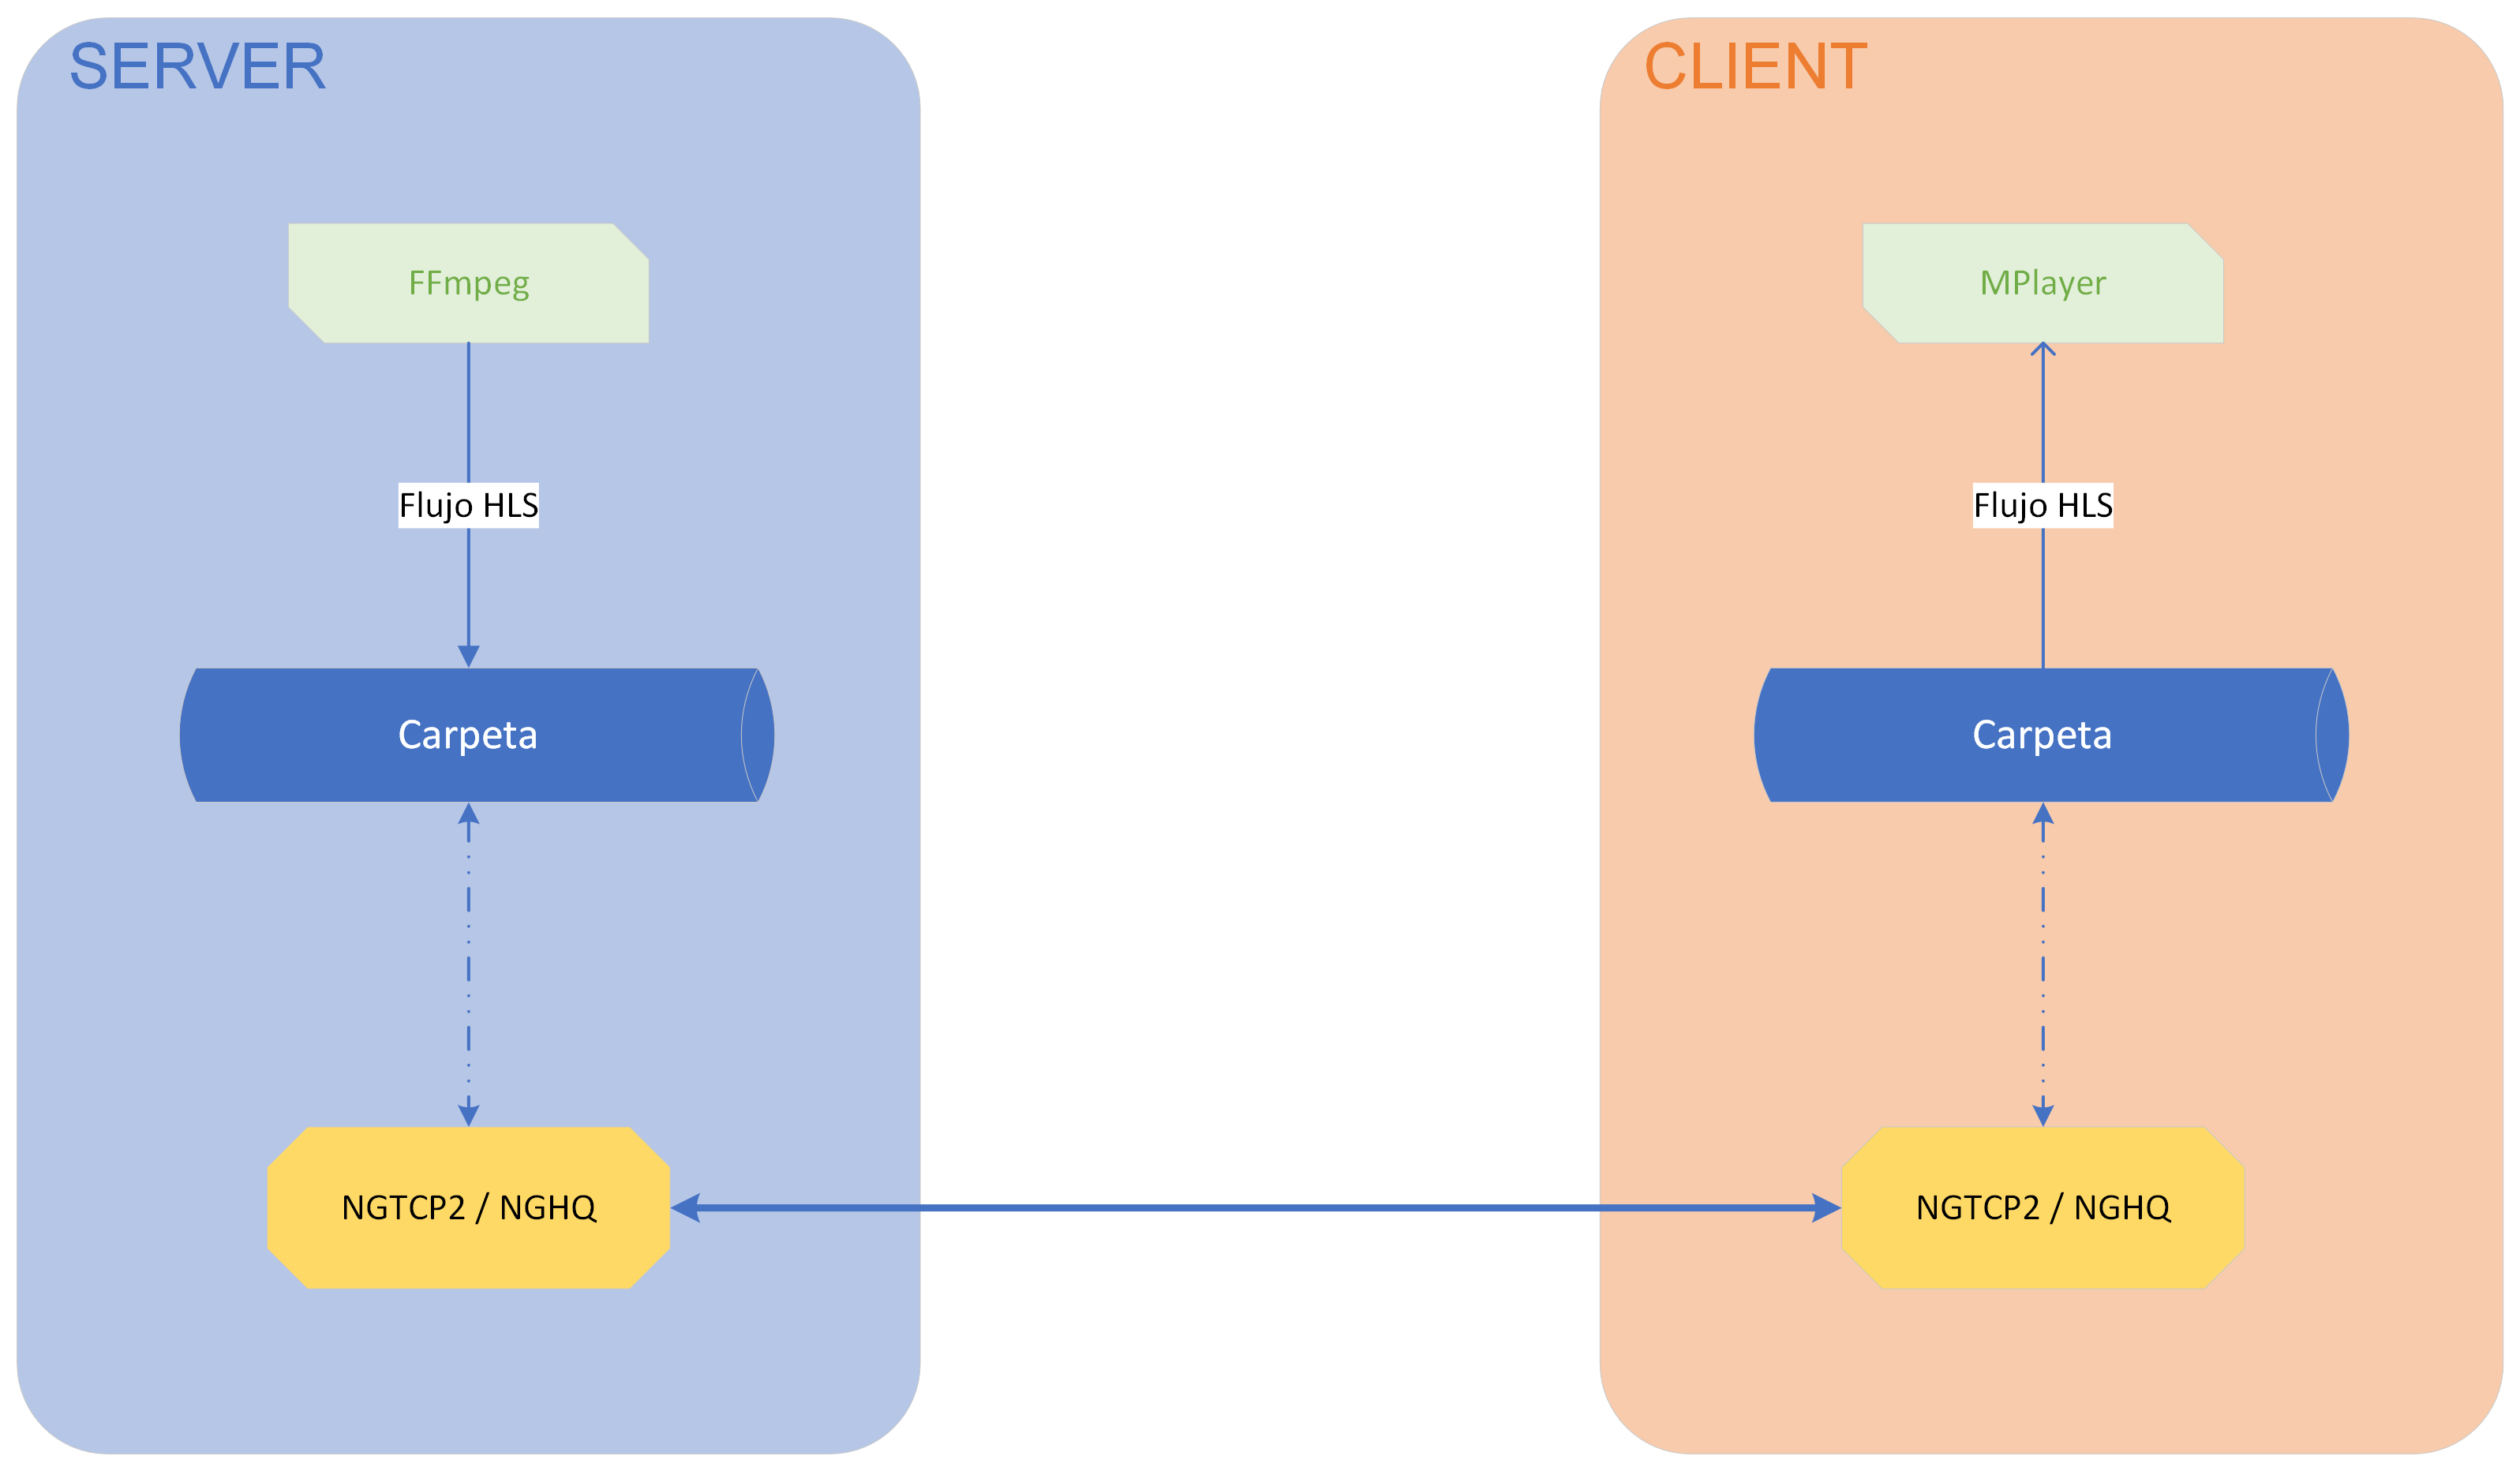
\includegraphics[width=15cm]{img/03_metodologia/system_design.png}
    \end{figure}
}
\subsubsection{Servidor}
{
    Per la banda del servidor, primer de tot es genera un fluxe de contingut amb \textit{ffmpeg} que es guarda en una 
    carpeta. Aquest fluxe és un video en bucle reproduit en temps real codificat en \ac{HLS}\footnote{És l'estàndar de
    codificació de video i audio utilitzat per transmetre contingut en temps real a Internet.}. Una vegada s'ha començat
    a crear el fluxe, aquest es detectat per un script creat en Python que anirà indicant continuament quan s'ha modificat
    l'arxiu de senyalització (.m3u8) i quin és l'últim troç de fluxe de dades creat (.ts).

    En el cas d'unicast, aquest ha de ser demanat pel client (GET) i en el cas de multicast aquest serà enviat directament
    a l'usuari (server Push).
}

\subsubsection{Client}
{
    Per la banda del client, el fluxe creat pel servidor serà rebut (multicast) o demanat (unicast). Aquest s'emmagatzemarà 
    en una carpeta segons vagin arribant. Per poder visualitzar el video live-streaming mentre va arribant es pot inicialitzar
    un reproductor com pot ser Mplayer. S'ha de pensar que l'arxiu de senyalització (.m3u8) està pensat perquè pugui ser modificat
    en temps real (on-the-fly), fet que permet de cara a l'usuari final veure un fluxe continu.
}

\subsection{Metodologia de les proves}
{
    Per una part s'analitza la quantitat de tràfic generat en el cas multicast i en el cas unicast (prova quantitativa) i,
    per altra part, s'analitzarà la qualitat del tràfic rebut mirant el video rebut (prova qualitativa). En el dos casos 
    es faràn les corresponents taules comparatives i comentaris pertinents.

    En el nostre cas, per falta de potència i perquè és un entorn simulat i no un entorn real, no es faràn proves de quin
    és el límit d'usuaris en el servidor unicast. Per la teoria, i pràctica, no té sentit mirar quin és el límit d'usuaris
    en el cas multicast.
}




%%% RESULTS: SECTIONS %%%

%%% SECTION3 %%%
\newpage

%%% TESTING %%%
\clearpage
%\vspace*{2cm}
\section{Experiments and results}
\label{sec:tests}
\lipsum[9]

%%% BUDGET %%%
\clearpage
\section{Budget}
{\selectlanguage{english}
\foreignlanguage{english}{Depending on the thesis scope this document should include:}}

%%% ENVIRONMENT %%%
\clearpage
\section[Environment Impact (Optional)]{{Environment Impact (Optional)}}

{Whether the tasks that have led to the realization of this thesis, as if its results have identifiable environmental
impact, describe it in this section.}

%%% CONCLUSIONS AND FUTURE %%%
\clearpage
\section{Conclusions}
\label{sec:conclusions}

\lipsum[4]

\lipsum[3]

\section{Future Work}
\label{sec:futwork}

\lipsum[10]

%%% BIBLIOGRAPHY %%%
\newpage

\medskip

%% Da problemas, solucionarlo
%\bibliographystyle{unsrt}
%\bibliography{bibliography.bib}

%%% ANNEX %%%
\clearpage
\newpage
\begin{appendices}

{Appendices may be included in your thesis but it is not a requirement.}

\end{appendices}

\end{document}
